%----------------------------------------------------------------------------
\chapter{Data processing}\label{sect:DataProcessing}
%----------------------------------------------------------------------------
\section{CNN and Daily Mail data}
%----------------------------------------------------------------------------
The most widely used dataset on the field of summarization is the \textit{CNN - Daily Mail dataset}. 
This dataset contains over 300,000 articles and their respective summaries from Daily Mail articles collected from June 2010 to April 2015 and CNN news collected from April 2007 until the end of April 2015. \cite{CNN_DM}

The only downside is that the summaries are not strictly extracted from the article hence there are expressions in the summaries that may not appear in the original article.

There are multiple preprocessed versions available on this dataset. I've used a dataset provided to me by \emph{G�bor Recski}, my former consultant, currently working at \textit{Apollo AI} as the head of AI.
This preprocessed dataset was in a jsonl format, each line containing a dictionary with the article and the highlights from that article and also the set of sentences from each article, that together give the highest achievable ROUGE score using the naive greedy method described in chapter~\ref{sect:Background}. I will reference these summaries as the extracted summary of an article.

\subsection{Example from the dataset}\label{subsect:example}
\textbox{\textbf{Article}

An American woman died aboard a cruise ship that docked at Rio de Janeiro on Tuesday, the same ship on which 86 passengers previously fell ill, according to the state-run Brazilian news agency, Agencia Brasil. The American tourist died aboard the MS Veendam, owned by cruise operator Holland America. Federal Police told Agencia Brasil that forensic doctors were investigating her death. The ship's doctors told police that the woman was elderly and suffered from diabetes and hypertension, according the agency. The other passengers came down with diarrhea prior to her death during an earlier part of the trip, the ship's doctors said. The Veendam left New York 36 days ago for a South America tour.

\textbf{Summary}

The elderly woman suffered from diabetes and hypertension, ship's doctors say

Previously, 86 passengers had fallen ill on the ship, Agencia Brasil says.

\textbf{Extracted summary}

An American woman died aboard a cruise ship that docked at Rio de Janeiro on Tuesday, the same ship on which 86 passengers previously fell ill, according to the state-run Brazilian news agency, Agencia Brasil. The American tourist died aboard the MS Veendam, owned by cruise operator Holland America. Federal Police told Agencia Brasil that forensic doctors were investigating her death. The ship's doctors told police that the woman was elderly and suffered from diabetes and hypertension, according the agency.
}

As you can see the extracted summary contains the four best sentences from the article.

This example is one of the shortest articles in the dataset, barely longer than its extracted summary.

%----------------------------------------------------------------------------
\section{Universal Dependencies}
%----------------------------------------------------------------------------
Before we discuss the data processing steps any further I need to clarify what Universal Dependencies are, and why are they useful.

\begin{figure}[!ht]
	\centering
	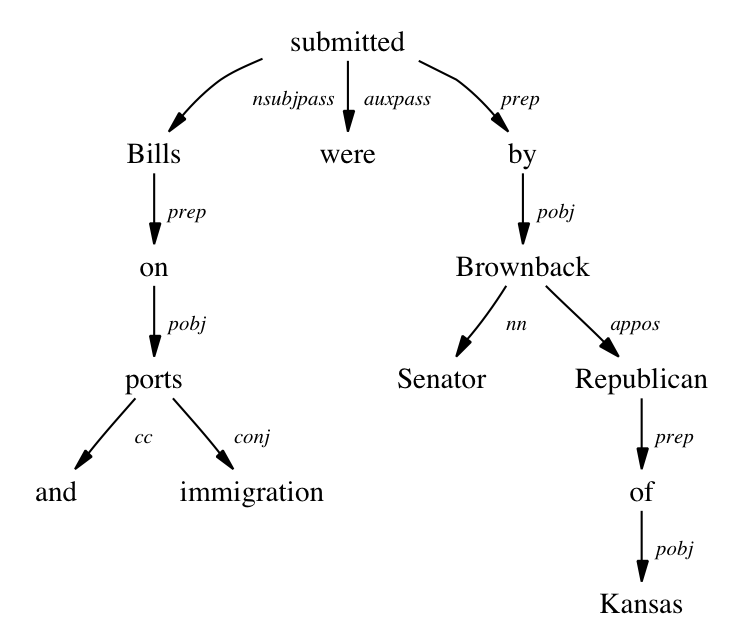
\includegraphics[width=100mm, keepaspectratio]{figures/UD.png}
	\caption{UD graph of Bills on ports and immigration were submitted by Senator Brownback, Republican of Kansas. Image from \href{https://nlp.stanford.edu/software/stanford-dependencies.shtml}{https://nlp.stanford.edu/software/stanford-dependencies.shtml}}
	\label{fig:UD}
\end{figure}

Universal dependency trees represent the grammatical relationships between the words of a sentence; it gives us the syntactic structure of the given sentence. They can be easily interpreted with some knowledge of the grammatical structure of languages and they are widely used because of this.

Dependency trees have been used from the early 20th century based on the work of Lucien Tesni\`ere. In his book titled \textit{\'El\'ements de syntaxe structurale} (Elements of Structural Syntax)\cite{UD} he described the modern grammatical dependency graph structure.

We construct these trees by dependency parsing. There is a multitude of ways we can do that, the library I used in my solution utilizes the deep learning based approach.

%----------------------------------------------------------------------------
\section{Graph format}
%----------------------------------------------------------------------------

The graph\_nets library uses a specific format for graphs, a so called GraphTuple. The user can transform multiple graphs with networkx format or dictionary format to a GraphTuple object. In my project I used dictionaries because they seemed to be the more straight forward and manageable approach.

The graph dictionary contains the following elements:
\begin{itemize}
	\item nodes: list containing the feature vectors of each node. In my final solution each node feature vector is the lemma and the part-of-speech tag of the given word 
	\item edges: list containing the feature vectors of each edge. The final feature vector contains the type of each word relation.
	\item globals: global parameter list. I found no relevant use for this parameter in my project.
	\item senders: list containing the indexes of the sender nodes in the order of the edges.
	\item receivers: list containing the indexes of the receiver nodes in the order of the edges.
\end{itemize}

\begin{figure}[!ht]
	\centering
	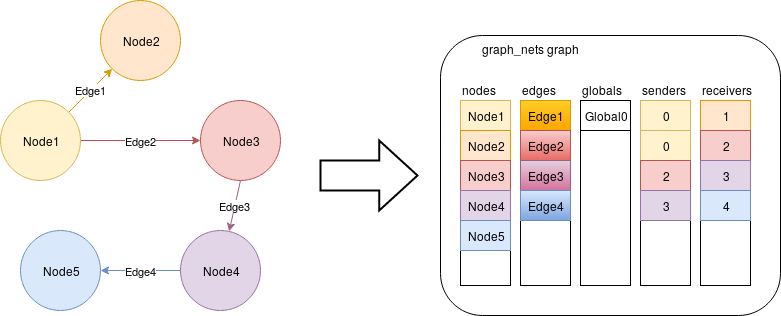
\includegraphics[width=150mm, keepaspectratio]{figures/transform_color.png}
	\caption{Graph transformation to dictionary format.}
	\label{fig:transform_graph}
\end{figure}

On the visual representation Figure \ref{fig:transform_graph} of this kind of graph transformation I highlighted the nodes and edges and the corresponding feature vectors and indexes with the same color for easy traceability.

Although I mentioned the transformation between one graph dictionary and one GraphTuble, but one instance of GraphTuple usually contains a batch of multiple graphs. To be able to handle multiple graphs the GraphTuple object has two more fields calculated during the transformation between the list of graph dictionaries and the GraphTuple instance:
\begin{itemize}
	\item n\_node: the number of nodes in each graph.
	\item n\_edge: the number of edges in each graph.
\end{itemize}

\begin{figure}[!ht]
	\centering
	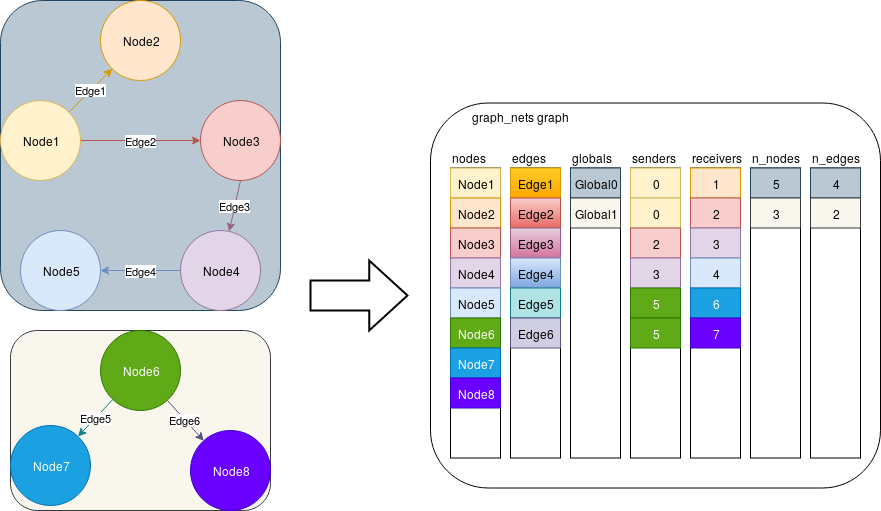
\includegraphics[width=150mm, keepaspectratio]{figures/transform_multiple.png}
	\caption{Graph transformation to GraphTuple format. The dictionary list is not visualized.}
	\label{fig:transform_multiple}
\end{figure}

On the Figure \ref{fig:transform_multiple} depicting this I also applied highlighting on the nodes, edges and graph backgrounds and the corresponding feature vectors and indexes with the same color.

%----------------------------------------------------------------------------
\section{Building the graphs}
%----------------------------------------------------------------------------

As I mentioned in the Introduction\ref{sect:Introduction} I used the stanfordnlp library to generate the universal dependency parse trees from the texts. Using the lemma and part of speech (POS) tag of the words I constructed the nodes of the graph the following way: if a word's lemma appears multiple times with the same POS tag in the text I've treated them as one node and the dependencies were merged as edges.

The feature vector of each node became their lemma and POS tag. The feature vector of the edges quite similarly is their UD relation type.

\begin{figure}[!ht]
	\centering
	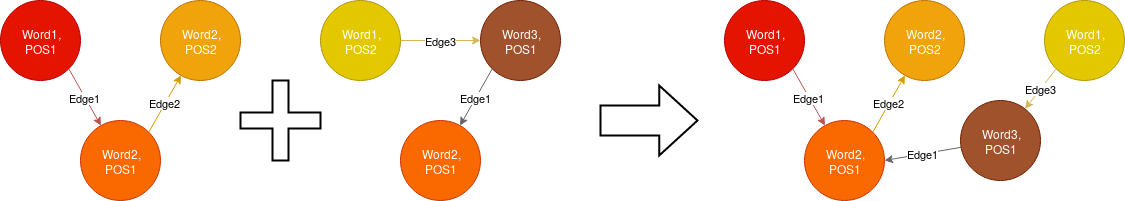
\includegraphics[width=150mm, keepaspectratio]{figures/merge_graphs_color.png}
	\caption{Graph merge.}
	\label{fig:merge_graph_color}
\end{figure}

\begin{figure}[!ht]
	\centering
	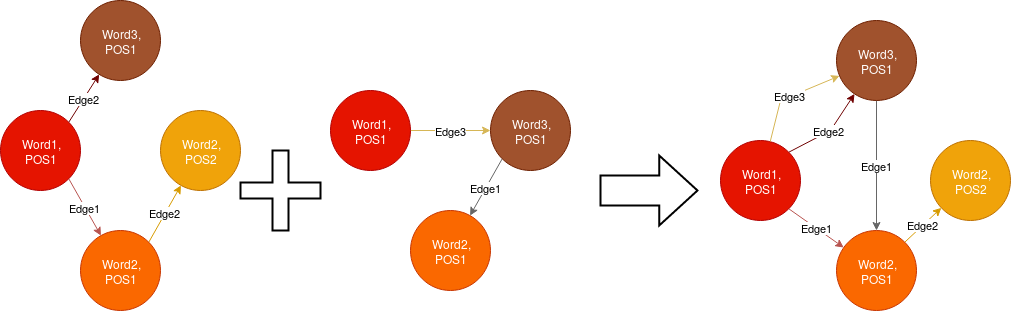
\includegraphics[width=150mm, keepaspectratio]{figures/merge_graphs_color_multiple.png}
	\caption{Graph merge with multiple matching nodes.}
	\label{fig:merge_graph_color_multiple}
\end{figure}

As you can see at Figure \ref{fig:merge_graph_color}, the resulting graph is not a correct UD graph because the \textit{Word2, POS1} node has multiple incoming edges.

On Figure \ref{fig:merge_graph_color_multiple} you can see how multiple node matches affect the construction of the graph merging.

With this method I was able to represent an article with one big graph, like the one on Figure \ref{fig:large_article_graph}. As you can see, it is not easily interpretable for a human at first glance, but you can tell, that the nodes with high connectivity appeared frequently. Most of these are stop-words, which I left in the graphs for the connectivity.

\begin{figure}[!ht]
	\centering
	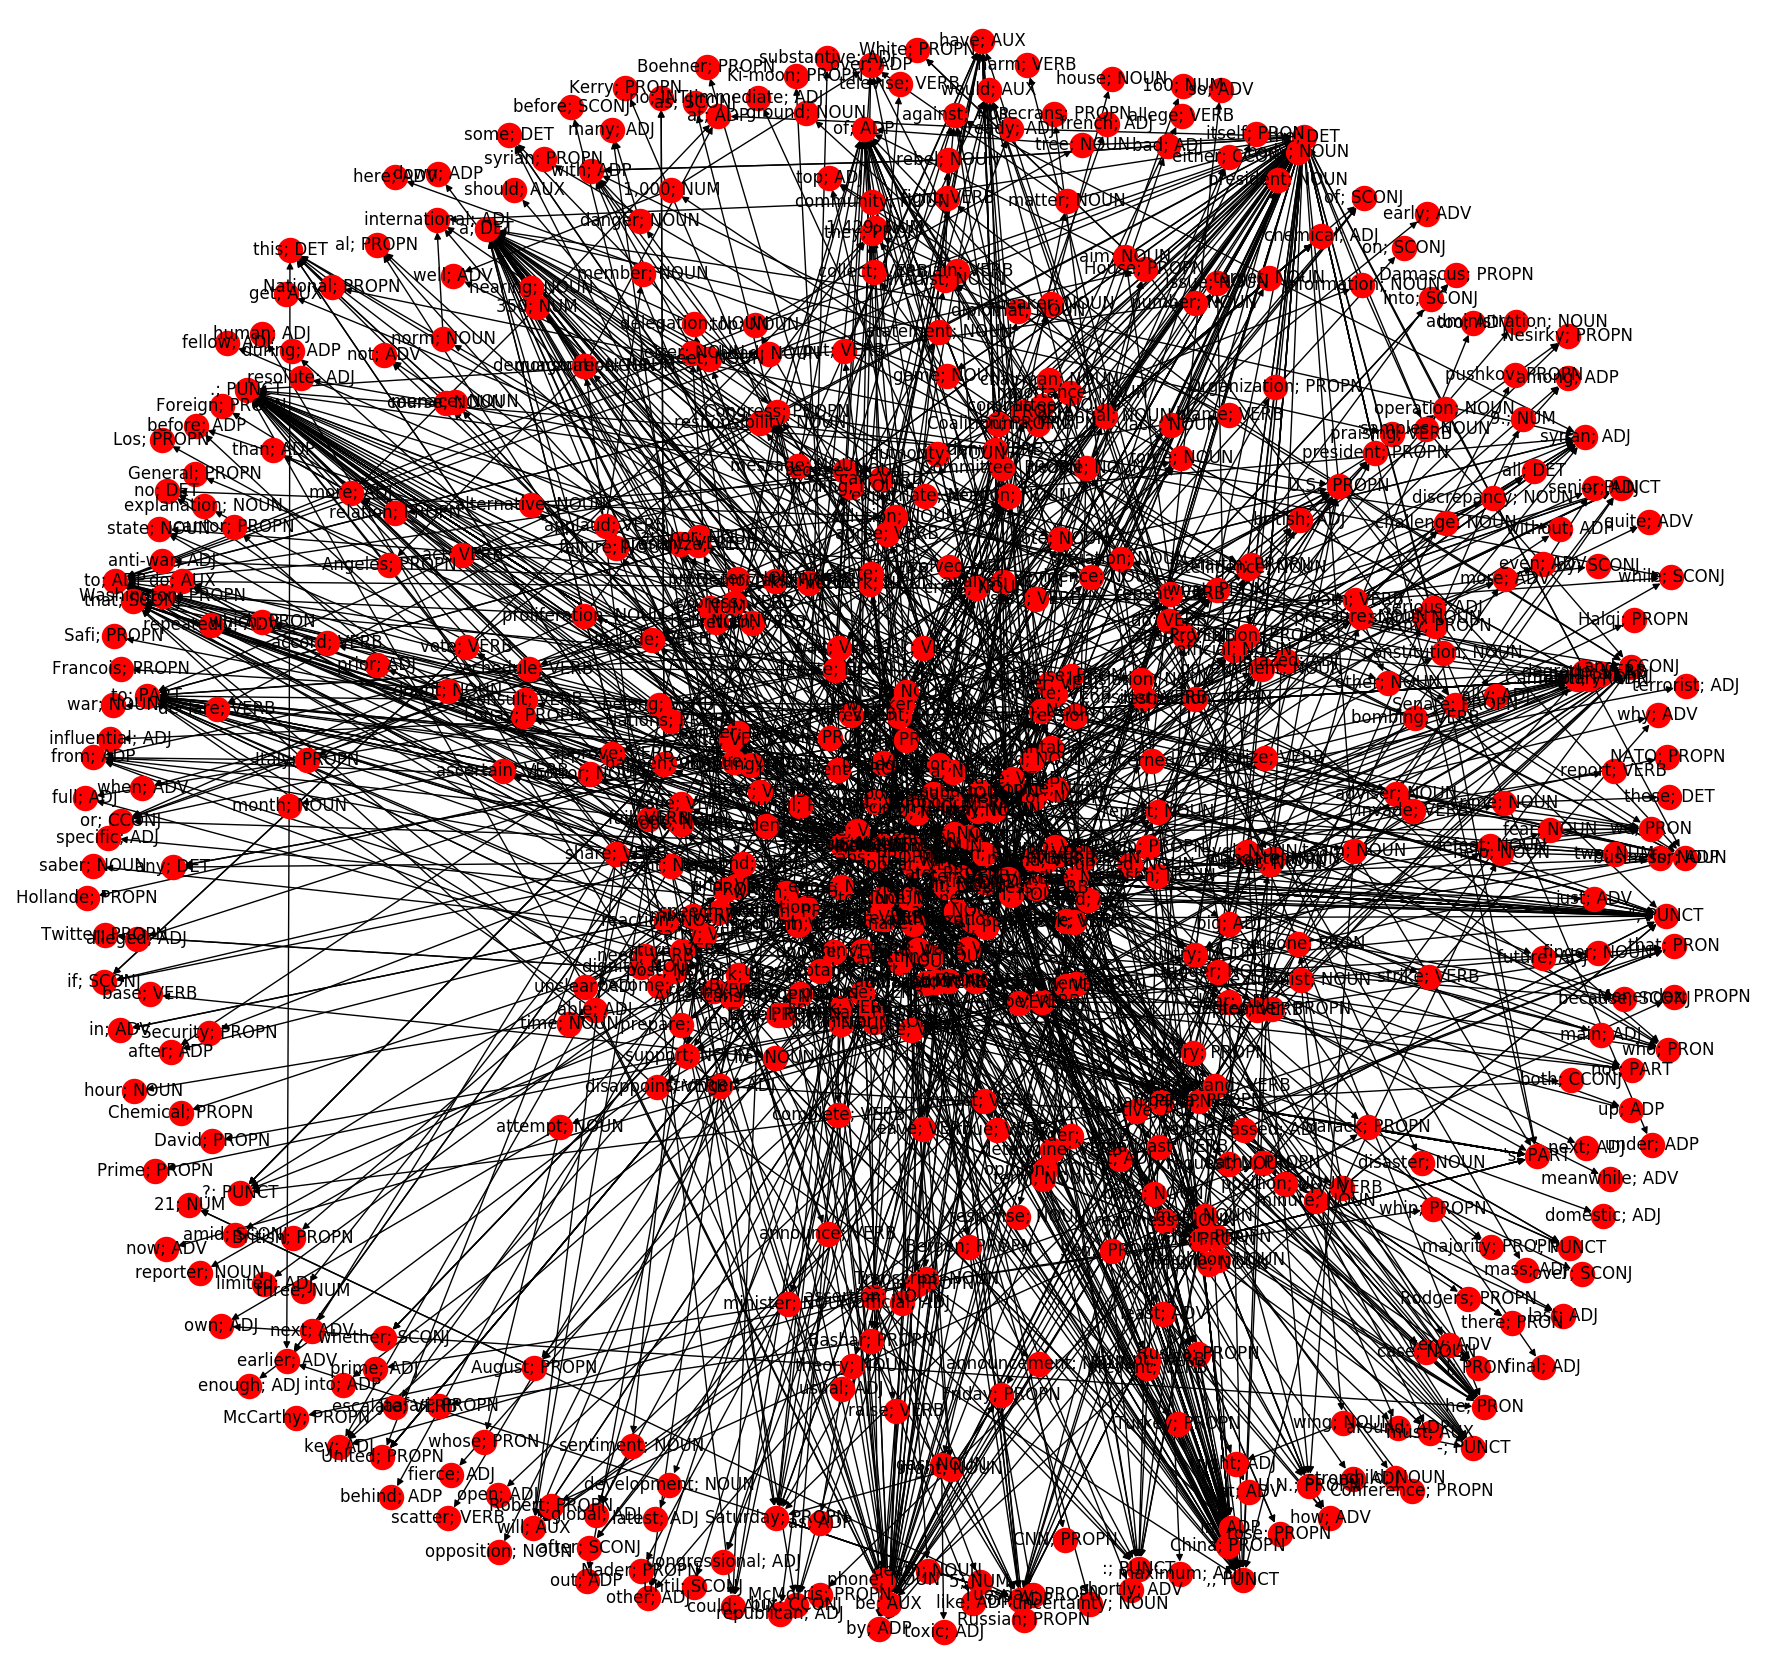
\includegraphics[width=150mm, keepaspectratio]{figures/large_article_graph.png}
	\caption{A normal length instance of article graph.}
	\label{fig:large_article_graph}
\end{figure}

\begin{figure}[!ht]
	\centering
	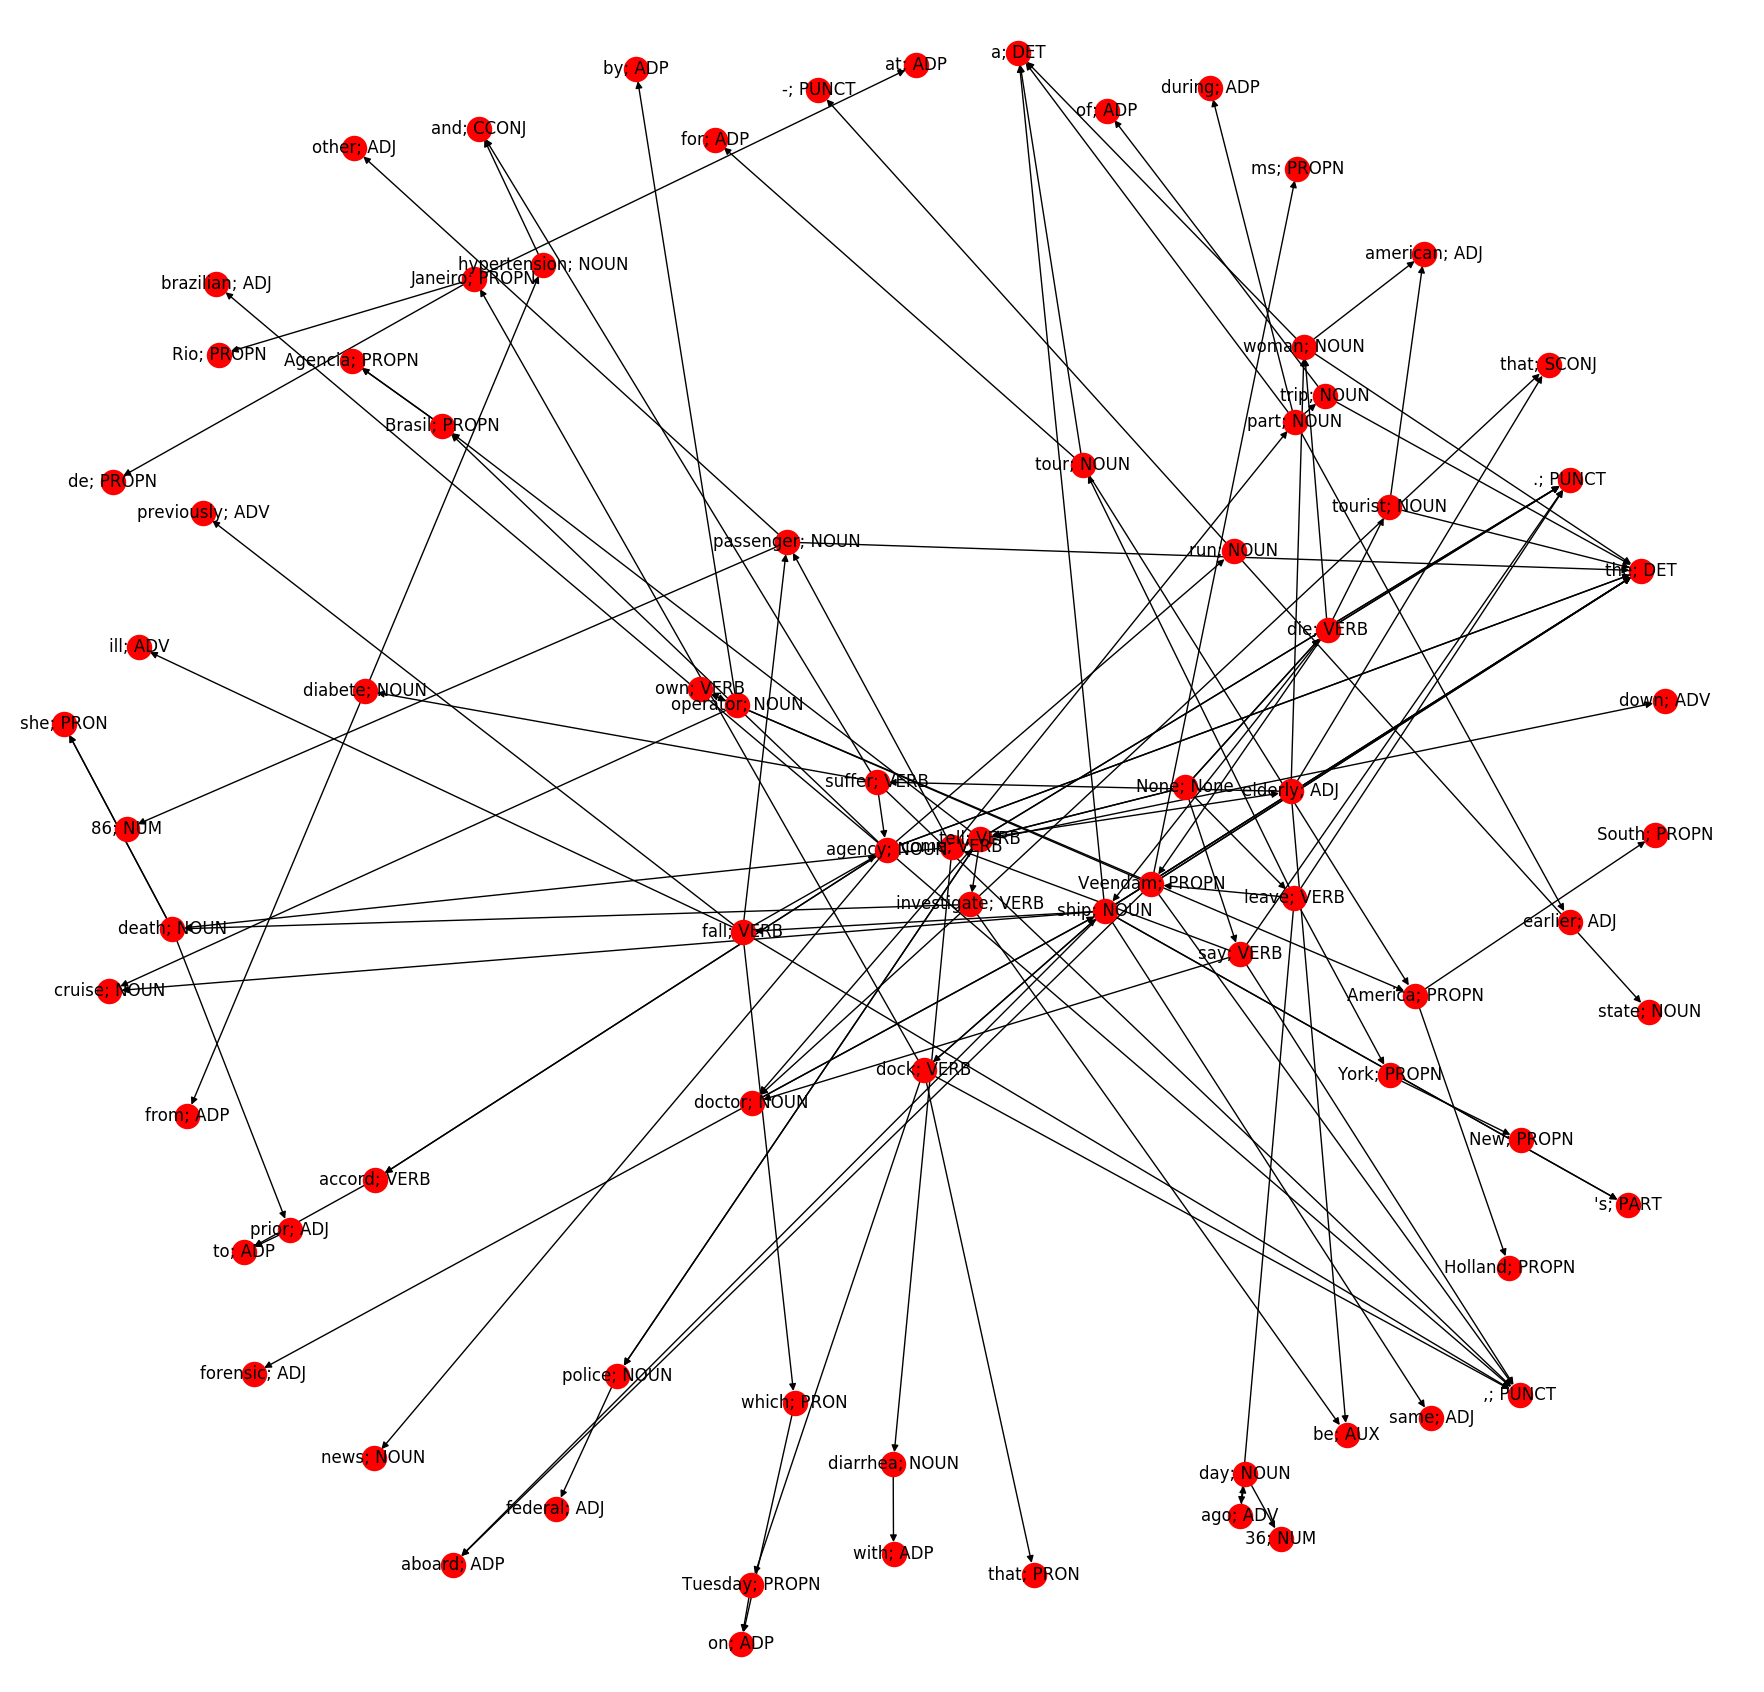
\includegraphics[width=150mm, keepaspectratio]{figures/small_article_graph.png}
	\caption{A short instance of article graph.}
	\label{fig:small_article_graph}
\end{figure}

The Figure \ref{fig:small_article_graph} is another example. It is the graph representation of the example in \ref{subsect:example}. It might be easier to understand, but it is not representative of the whole dataset due to its shortness.

%----------------------------------------------------------------------------
\section{Forming the target graphs}
%----------------------------------------------------------------------------
Initially my approach was to try to learn the summaries written by people. For this I needed to generate summary graphs, but their structure was not adequate for training any graph neural network on it. So my solution was the following: I iterated through the edges of the article graph and if the sender node, the receiver node and the edge type matched any edge in the summary I've marked them by adding a 1.0 at the end of their feature vector. Otherwise I appended a 0.0 to the vector.

Similarly I iterated through the nodes as well and checked whether the same feature vector appears in the summary graph and appended 1.0 in case of successful search, 0.0 otherwise.

This way I was able to achieve the same structure, but with marked summary nodes and edges.

The problem with this approach was the fact, that some of the expressions used in the summary did not match up with anything from the original text so the result could not contain the same level of information as the summary graph on it's own.

However after I received the dataset that contained the extracted summaries with the best possible ROUGE score I was able to use that as the expected output of my neural network. The construction is similar to the previous one, but instead of generating an other graph and then trying to find the corresponding parts I only iterated through the ud graphs b sentences and labeled the nodes and edges in that with the right label.

\begin{figure}[!ht]
	\centering
	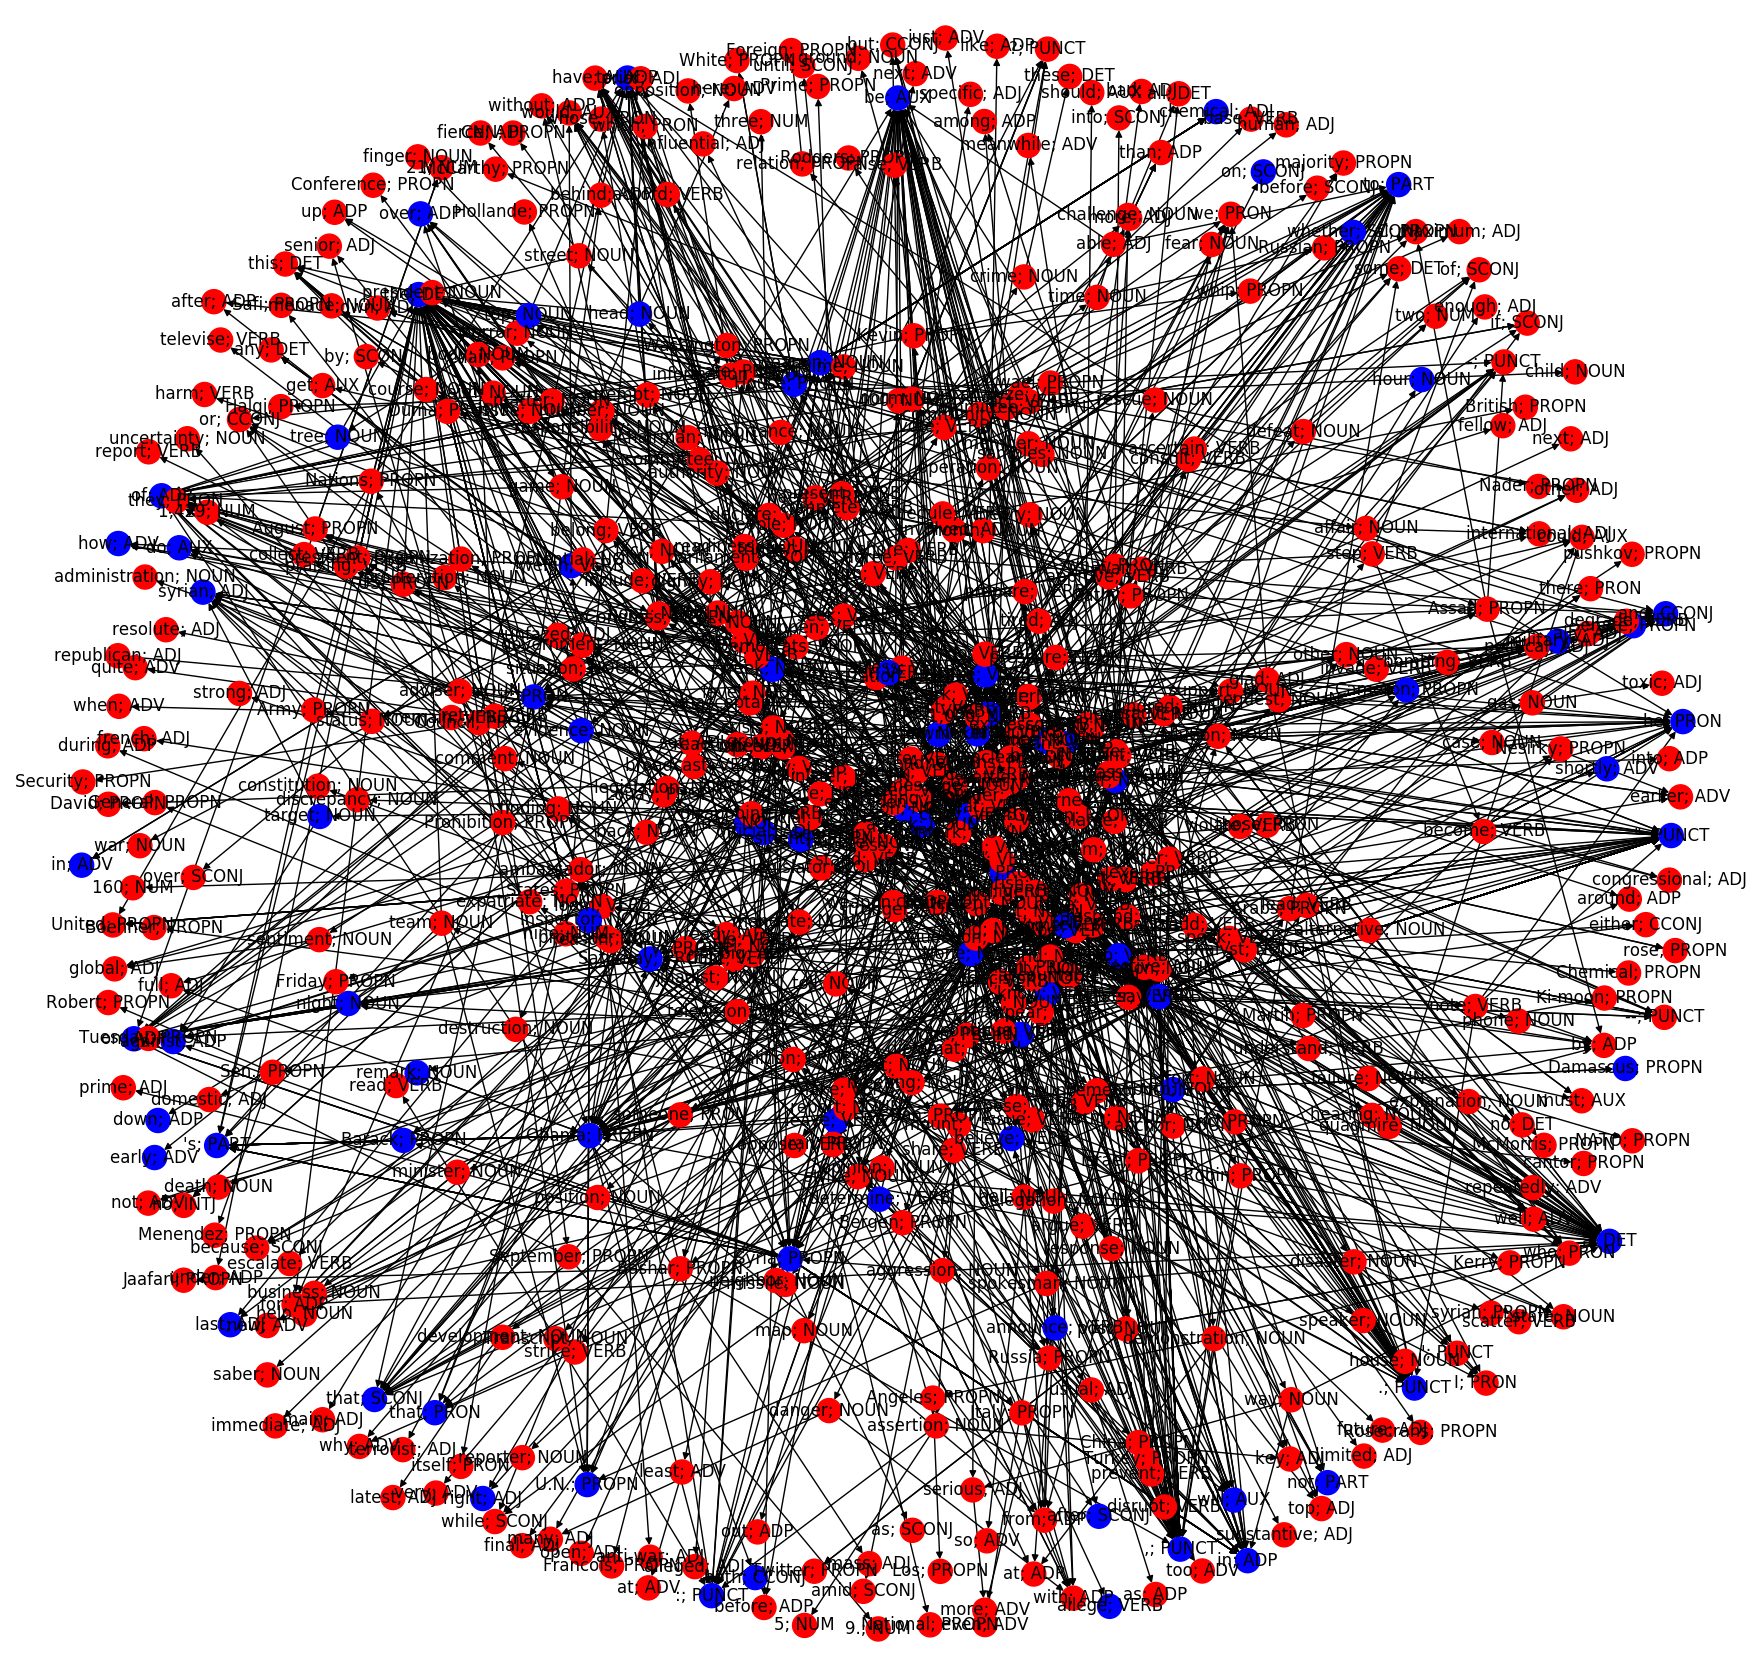
\includegraphics[width=150mm, keepaspectratio]{figures/large_article_graph_color.png}
	\caption{The colored article graph of the normal length article. I highlighted the nodes with label 1 with blue.}
	\label{fig:large_article_graph_colored}
\end{figure}

\begin{figure}[!ht]
	\centering
	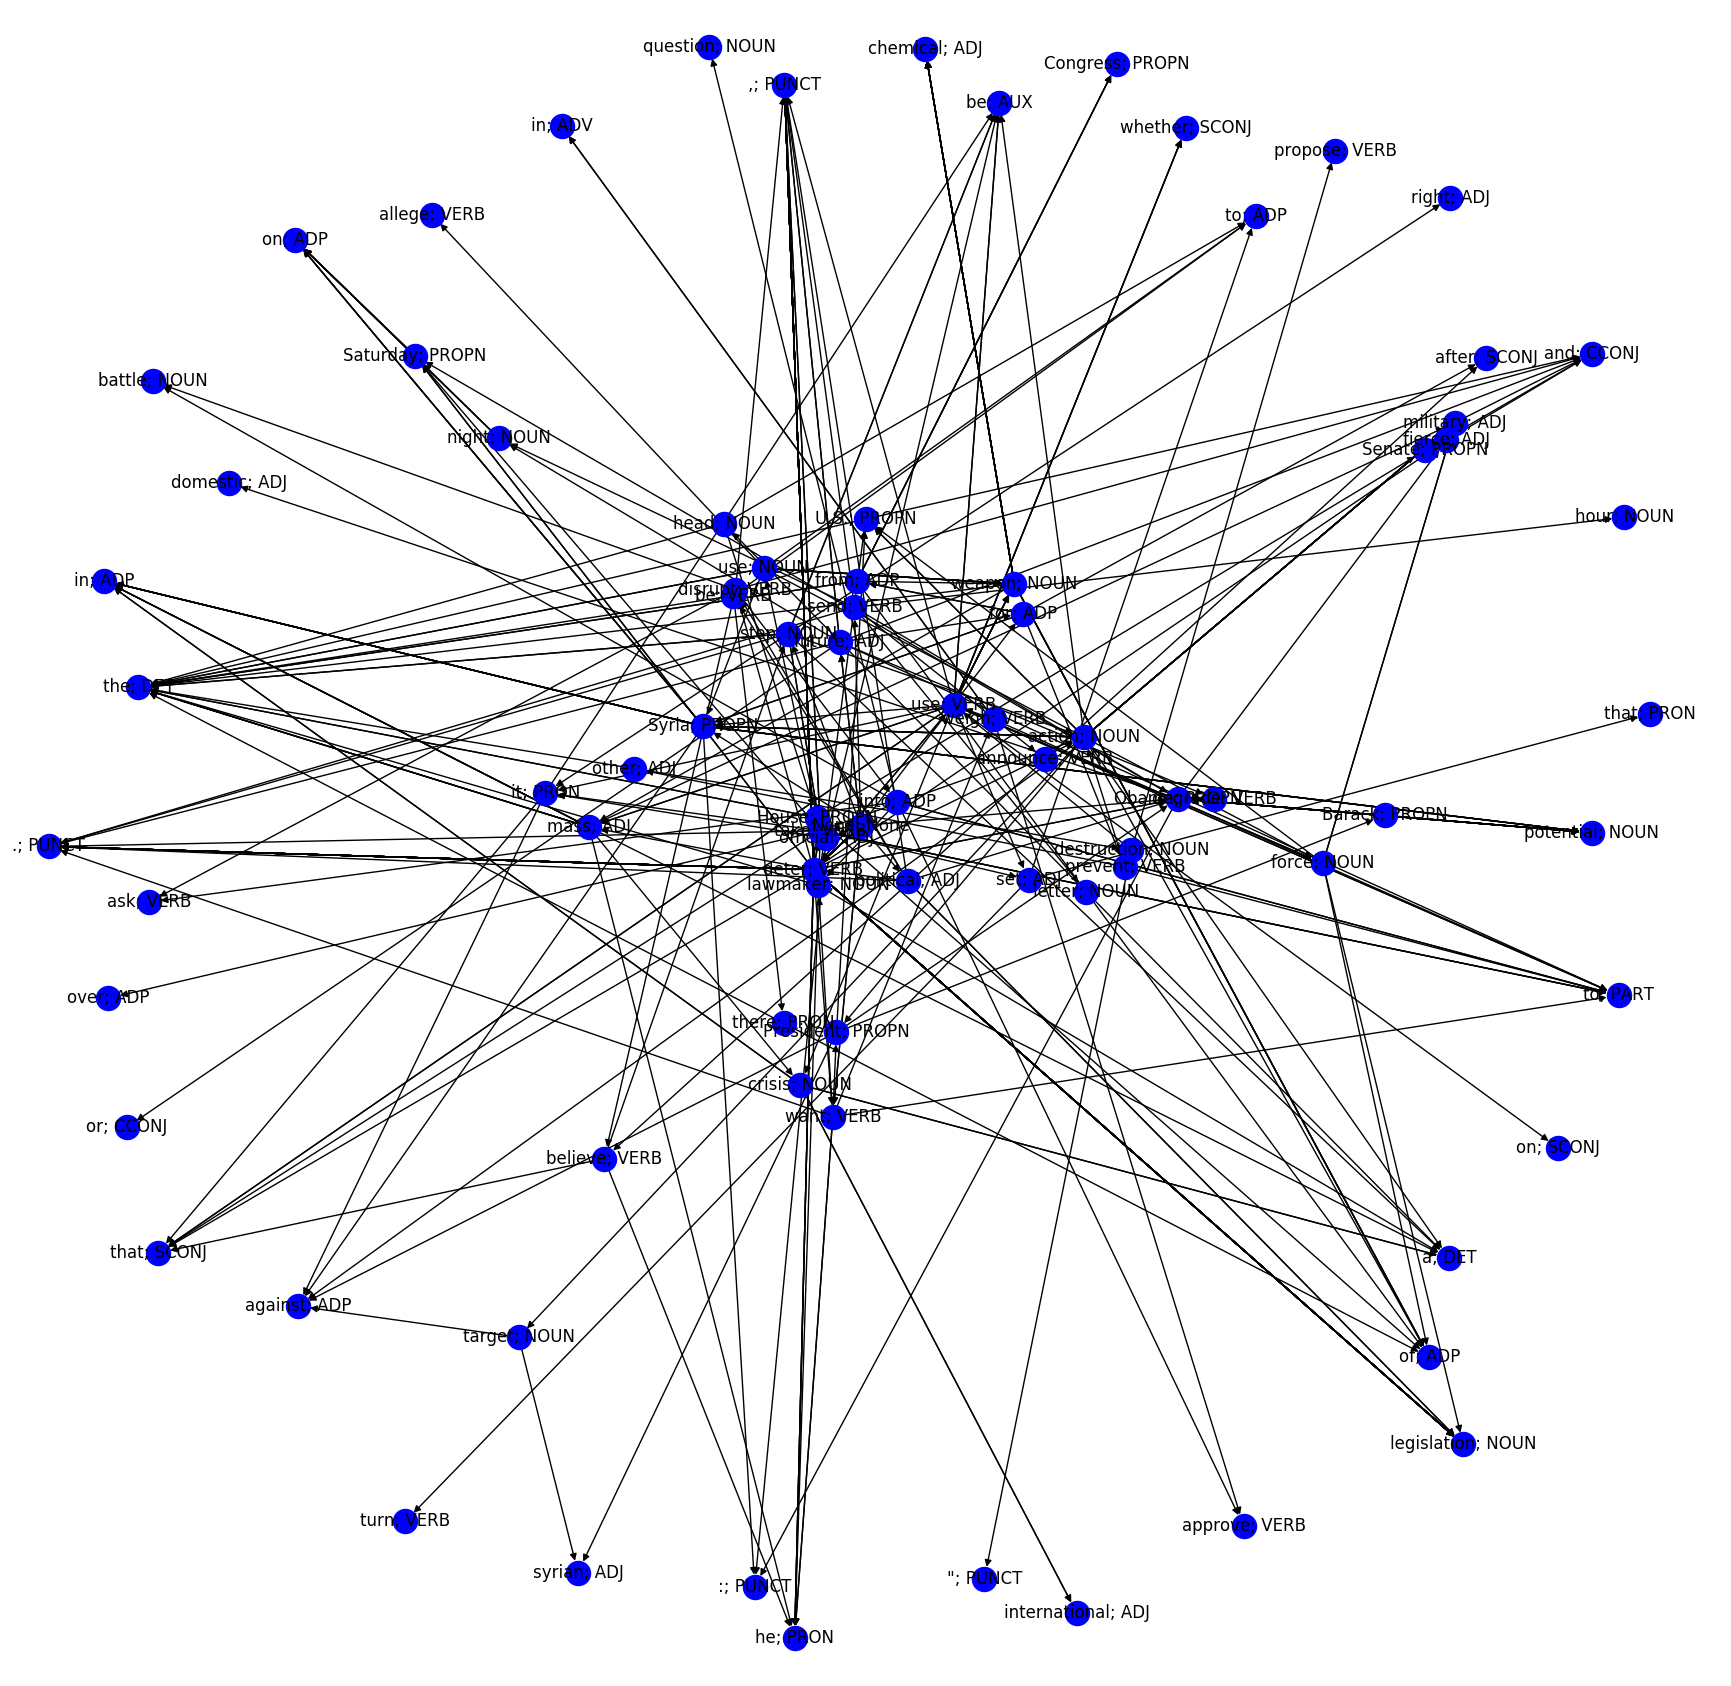
\includegraphics[width=150mm, keepaspectratio]{figures/large_summary_graph.png}
	\caption{The summary graph of the normal length article. This is the subgraph of the article graph with the node labels of 1.}
	\label{fig:large_summary_graph}
\end{figure}


\begin{figure}[!ht]
	\centering
	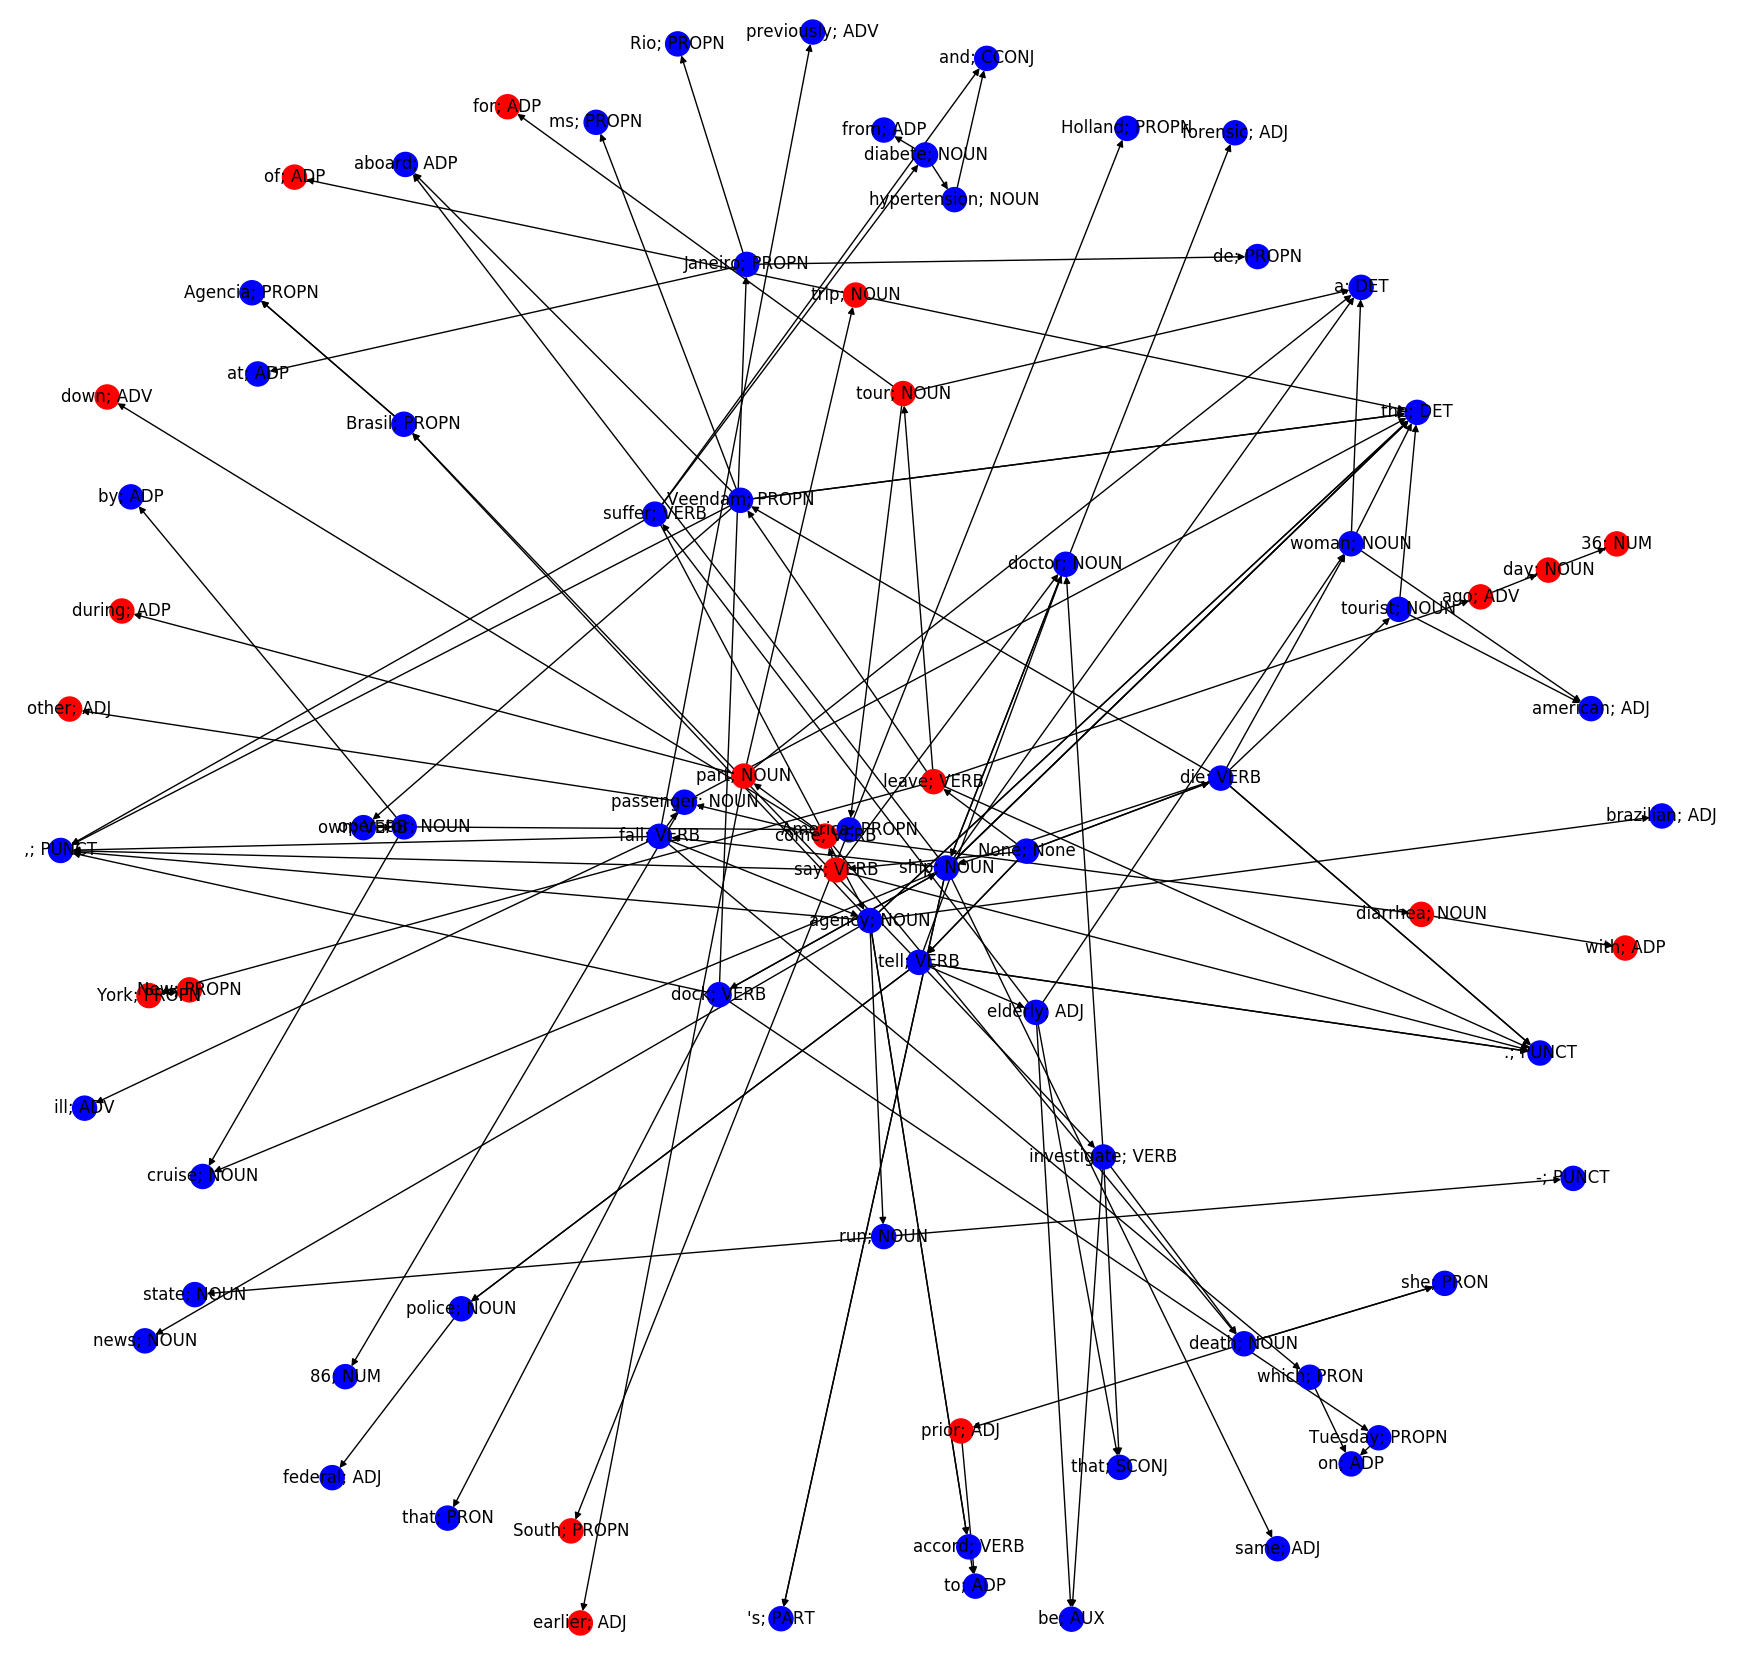
\includegraphics[width=150mm, keepaspectratio]{figures/small_article_graph_color.png}
	\caption{The colored article graph of the short article. I highlighted the nodes with label 1 with blue.}
	\label{fig:small_article_graph_colored}
\end{figure}

\begin{figure}[!ht]
	\centering
	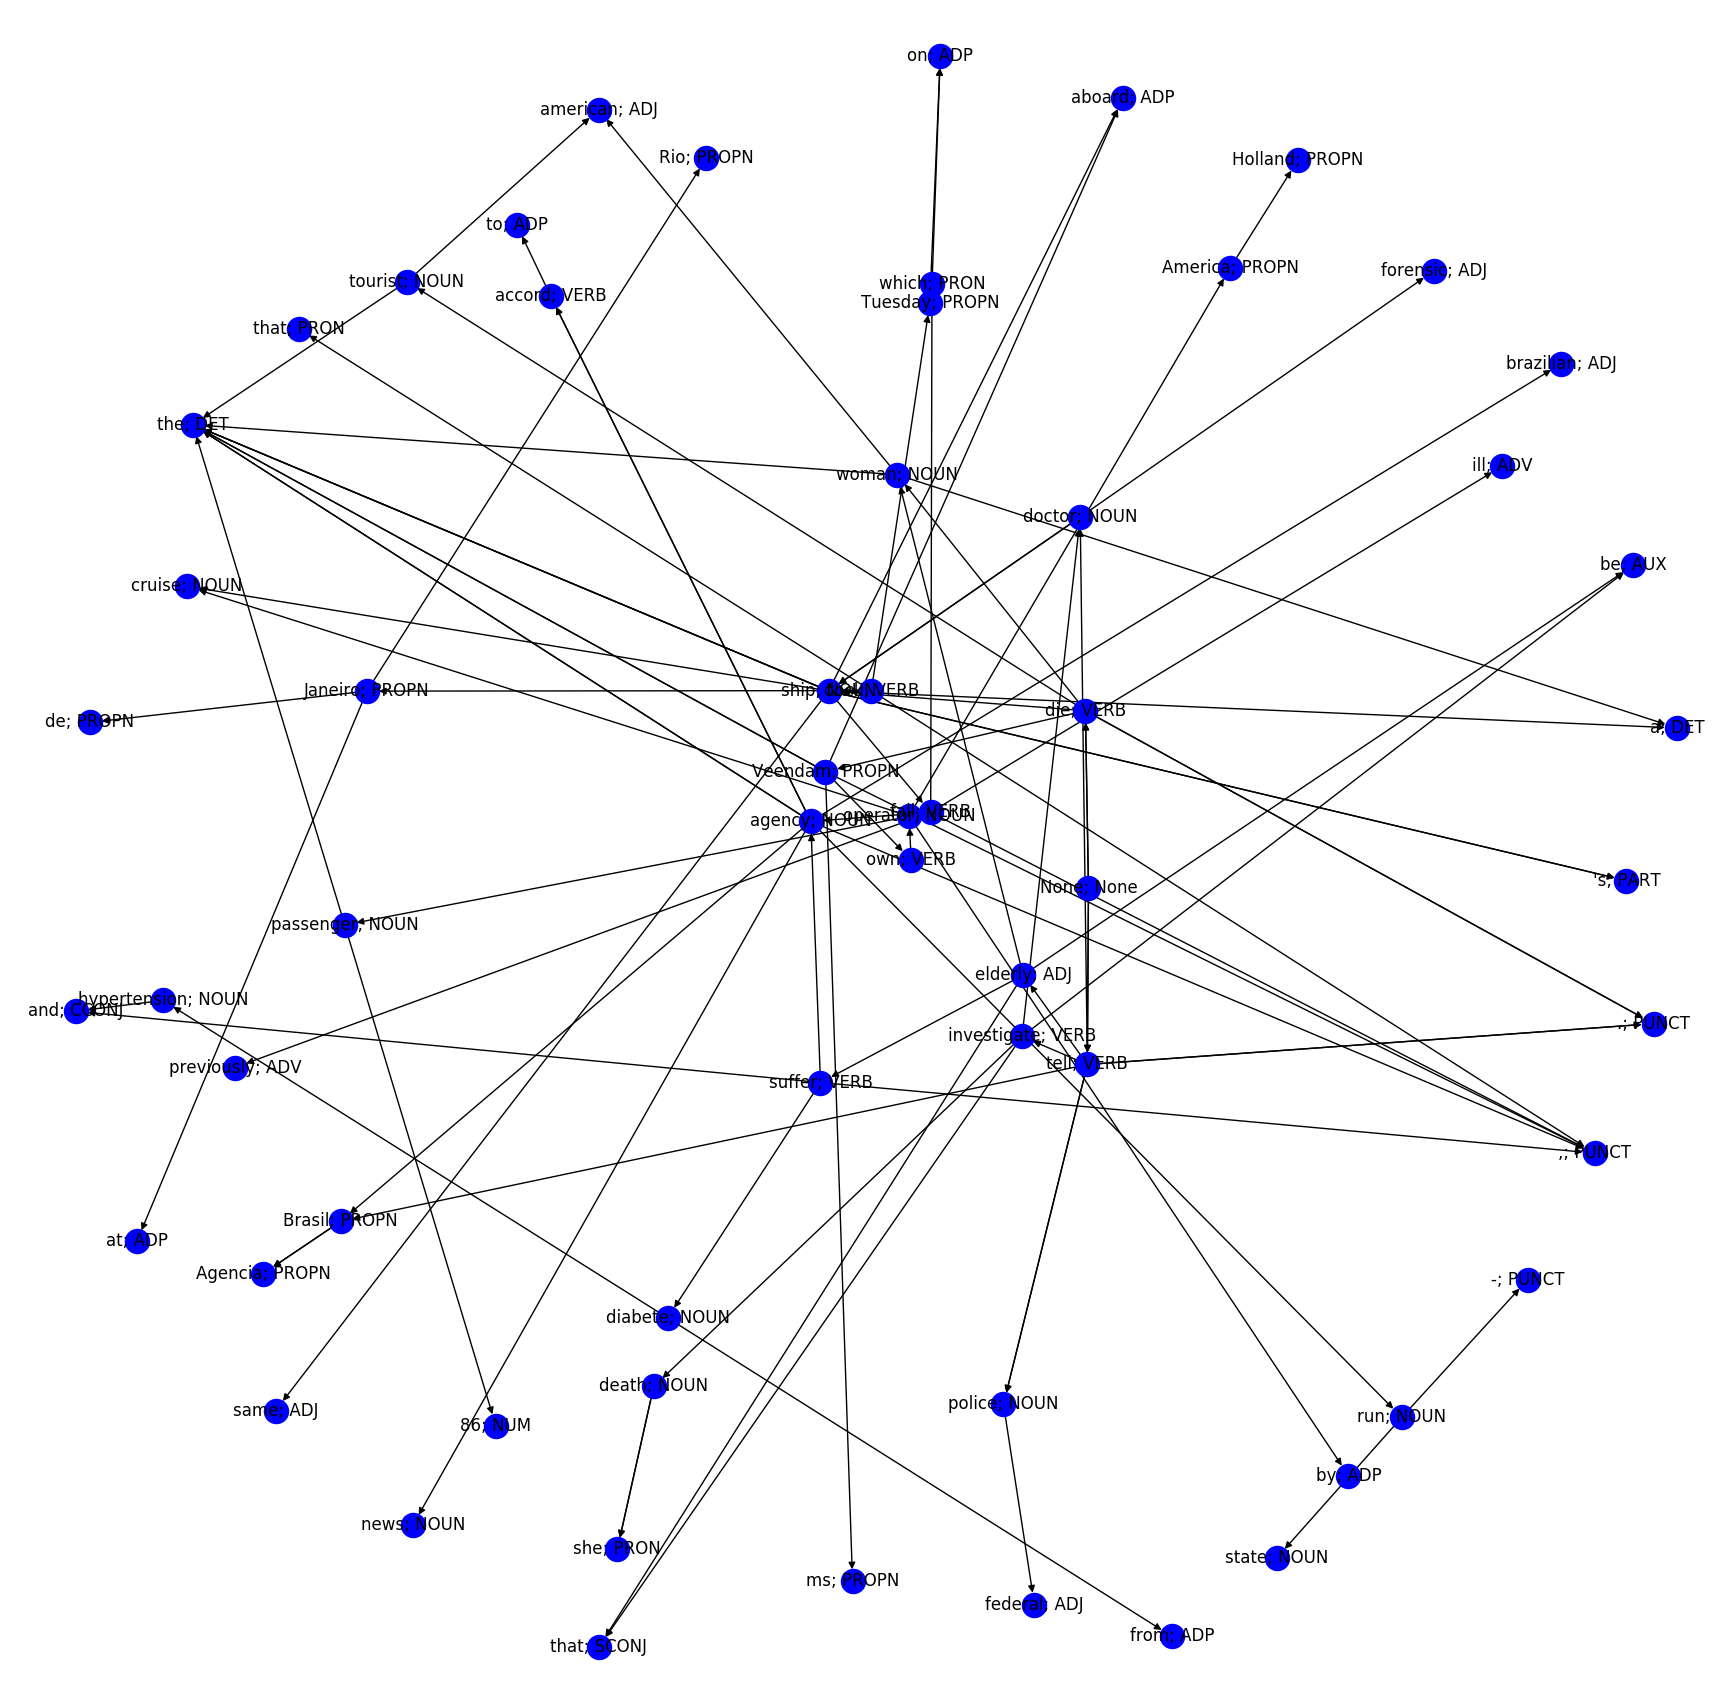
\includegraphics[width=150mm, keepaspectratio]{figures/small_summary_graph.png}
	\caption{The summary graph of the short article. This is the subgraph of the article graph with the node labels of 1.}
	\label{fig:small_summary_graph}
\end{figure}
The graphs resulting from this approach contained more information and proved better for training. On Figure \ref{fig:large_article_graph_colored} and Figure \ref{fig:large_summary_graph} you can see the results of the first article visualized in two different ways and on Figure \ref{fig:small_article_graph_colored} and Figure \ref{fig:small_summary_graph} the results of the short article.
